\documentclass{article}
%\VignetteIndexEntry{catenary}
\author{Jono Tuke \& Matt Roughan}
\title{Getting started with the {\tt catenary} package }
\usepackage{Sweave}
\begin{document}
\Sconcordance{concordance:catenary.tex:catenary.Rnw:%
1 4 1 1 0 13 1 1 2 1 0 2 1 4 0 1 2 1 1 1 2 1 0 1 1 4 0 1 2 16 1 1 2 6 0 %
1 1 6 0 1 1 7 0 1 1 22 0 1 2 3 1 1 2 1 0 3 1 7 0 1 1 6 0 1 1 4 0 1 3 6 %
0 1 1 4 0 1 3 6 0 1 1 4 0 1 2 2 1 1 2 1 0 2 1 5 0 1 1 27 0 2 2 5 0 1 2 %
28 1}

\maketitle

\section{Introduction}
The {\tt catenary} package has been created to let you fit catenaries to observed data, and also to explore how the parameter values of a catenary affects its properties. There are two main classes in the {\tt catenary} package: the {\tt catenary} class and the {\tt fittedCatenary}. 

Recall that the general form of the catenary has three parameters: $c_1,c_2,\lambda$ and is of the form:
\[
 y = c_1  \cosh\left( \frac{x-c_2}{c_1} \right) + \lambda
\]

\section{ Exploring catenaries with parameter values}
A {\tt catenary} object can be created given the values of $c_1, c_2, $ and $\lambda$ as follows:
\begin{Schunk}
\begin{Sinput}
> library(catenary)
> cat1 <- catenary(c1=1,c2=2,lambda=3,x0=0,x1=4)
> plot(cat1)
\end{Sinput}
\end{Schunk}
\includegraphics{catenary-001}

You can also get inverted catenaries
\begin{Schunk}
\begin{Sinput}
> cat2 <- catenary(c1=-1,c2=2,lambda=3,x0=0,x1=4)
> plot(cat2)
\end{Sinput}
\end{Schunk}
\includegraphics{catenary-002}

As well as the {\tt plot()} function, the following functions are available (Table~\ref{tab:functions}).

\begin{center}
\begin{table}
\begin{tabular}{l|r}
Function name & what it does \\\hline
{\tt L} & gives length of catenary\\
{\tt vertex} & gives x and y coordinates of vertex\\
{\tt minmax} & gives min and max values of y of the catenary\\
{\tt Summary} & bit of everything
\end{tabular}
\caption{{\tt catenary} functions}
\label{tab:functions}
\end{table}
\end{center}

\begin{Schunk}
\begin{Sinput}
> L(cat1)
\end{Sinput}
\begin{Soutput}
[1] 7.253721
\end{Soutput}
\begin{Sinput}
> vertex(cat1)
\end{Sinput}
\begin{Soutput}
x y 
2 4 
\end{Soutput}
\begin{Sinput}
> minmax(cat1)
\end{Sinput}
\begin{Soutput}
    x        y
min 2 4.000000
max 0 6.762196
\end{Soutput}
\begin{Sinput}
> Summary(cat1)
\end{Sinput}
\begin{Soutput}
$parameters
       value
c1         1
c2         2
lambda     3

$endpoints
      x        y
left  0 6.762196
right 4 6.762196

$length
[1] 7.253721

$vertex
x y 
2 4 
\end{Soutput}
\end{Schunk}

\section{ Exploring catenaries with just the endpoints}
Alternatively, you can define a catenary by giving its endpoints and length. If you do not give a length, then you can ask for the natural catenary based on ??(Matt info needed) or the maximum catenary, i.e., the one that just touches the ground

\begin{Schunk}
\begin{Sinput}
> left <- c(-2,1)
> right <- c(2,1)
> endpoints <- rbind(left,right)
> endpoints
\end{Sinput}
\begin{Soutput}
      [,1] [,2]
left    -2    1
right    2    1
\end{Soutput}
\begin{Sinput}
> cat3 <- catenary(endpoints=endpoints,L=5)
\end{Sinput}
\begin{Soutput}
Optim worked
uniroot worked
\end{Soutput}
\begin{Sinput}
> plot(cat3)
\end{Sinput}
\end{Schunk}
\includegraphics{catenary-004}
\begin{Schunk}
\begin{Sinput}
> cat4 <- catenary(endpoints=endpoints,type="natural")
\end{Sinput}
\begin{Soutput}
Optim worked
\end{Soutput}
\begin{Sinput}
> plot(cat4)
\end{Sinput}
\end{Schunk}
\includegraphics{catenary-005}
\begin{Schunk}
\begin{Sinput}
> cat5 <- catenary(endpoints=endpoints,type="max")
\end{Sinput}
\begin{Soutput}
Optim worked
\end{Soutput}
\begin{Sinput}
> plot(cat5)
\end{Sinput}
\end{Schunk}
\includegraphics{catenary-006}

\section{Fitting catenaries to data}
You can also fit a catenary to observed values of x and y. This will also fit a parabola. It also gives an indication of possible curves based on bootstrap refitting. 
\begin{Schunk}
\begin{Sinput}
> x <- runif(100,0,4)
> y <- f(x=x,c1=1,c2=2,lambda=3) + rnorm(100)
> cat6 <- fittedCatenary(x=x,y=y,R=100)
\end{Sinput}
\begin{Soutput}
[1] "Fitted catenary"
\end{Soutput}
\begin{Sinput}
> Summary(cat6)
\end{Sinput}
\begin{Soutput}
$parameters
           value
c1     0.9667921
c2     2.1172960
lambda 3.0161623

$endpoints
               x       y
left  0.05403083 7.15794
right 3.98877244 6.43552

$length
      c1 
7.307197 

$vertex
    x.c2     y.c1 
2.117296 3.982954 

$fits
    para catenary 
93.95937 97.91466 
\end{Soutput}
\end{Schunk}

\begin{Schunk}
\begin{Sinput}
> plot(cat6,fit=c("para","cat"),envelope=c("para","cat"))
\end{Sinput}
\end{Schunk}
\includegraphics{catenary-008}


As the class {\tt fittedCatenary} inherits from the class {\tt catenary} you get all the functions in Table~\ref{tab:functions}
\section{Ctesiphon data}
The Ctesiphon data is obtained from the photo shown in Figure~\ref{fig:ctesiphon}. From this points were selected from the internal and external arch (see Figure~\ref{internal} and Figure~\ref{external} respectively)

\begin{figure}[htpb]
  \begin{center}
		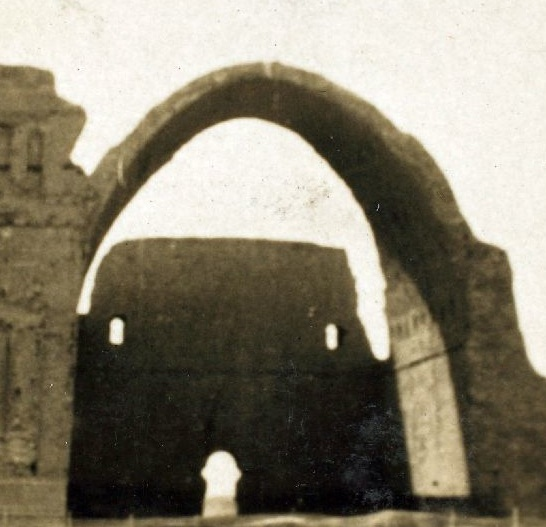
\includegraphics[width=\textwidth]{ctesiphon}
	\end{center}
	\caption{Ctesiphon.}
	\label{fig:ctesiphon}
\end{figure}
\begin{figure}[htpb]
  \begin{center}
		\includegraphics[width=\textwidth]{ctesiphon_internal}
	\end{center}
	\caption{Internal points for Ctesiphon.}
	\label{fig:internal}
\end{figure}
\begin{figure}[htpb]
  \begin{center}
		\includegraphics[width=\textwidth]{ctesiphon_external}
	\end{center}
	\caption{External points for Ctesiphon.}
	\label{fig:external}
\end{figure}

\end{document}
